\chapter{Rover Post-Development}
\label{chap:roverPostDev}
  \section{Final Product}
    Figures~\ref{fig:postDev-finalFull} and \ref{fig:postDev-finalViews} show the fully assembled rover model taken before the testing phase of the project.
    
    \begin{figure}[h!]
      \centering
      \includegraphics[width=0.9\linewidth]{figures/postDev-finalFull}
      \caption[Image of the front-left corner of the completed model of the rover.]{Image of the front-left corner of the completed model of the rover.}
      \label{fig:postDev-finalFull}
    \end{figure}
    
    \begin{figure}[H]
      \centering
      \subfloat[Rear view.]{
        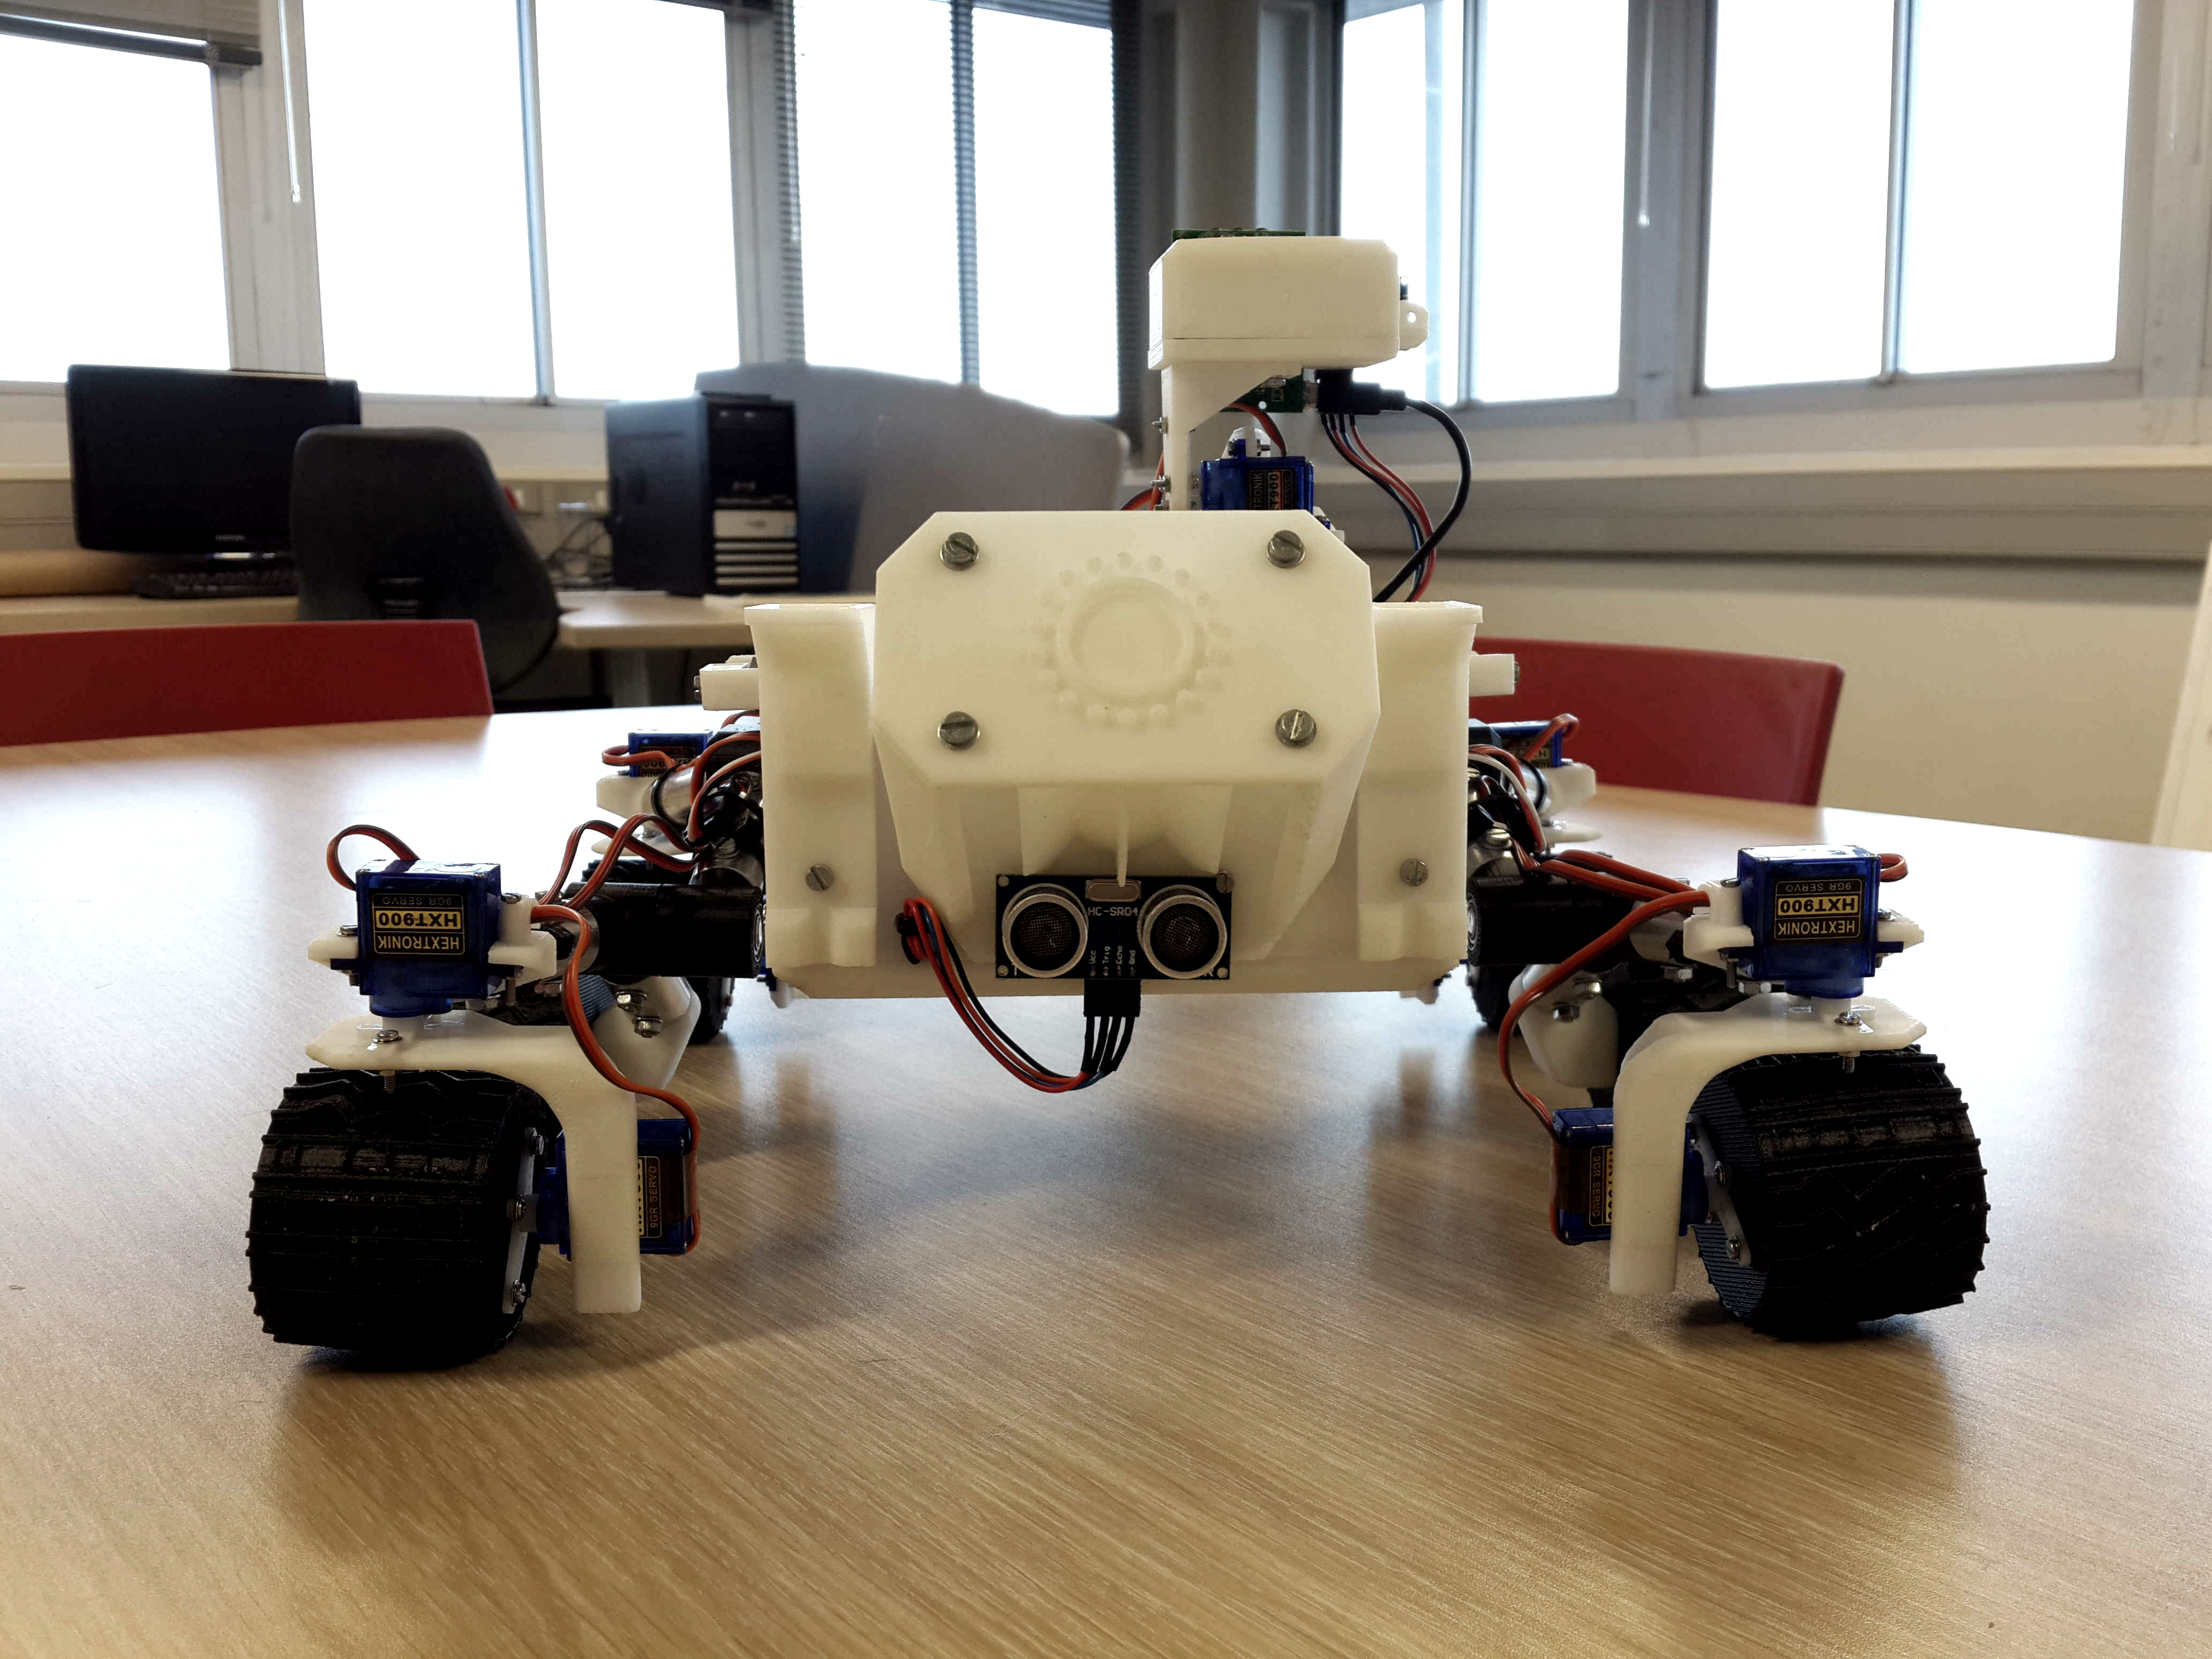
\includegraphics[width=.47\linewidth]{figures/postDev-fullRear.jpg}
      }%
      \subfloat[Side view.]{
        \includegraphics[width=.47\linewidth]{figures/postDev-fullSide.jpg}
      }
      \caption[Images of the completed model of the rover from two additional angles.]{Images of the completed model of the rover from two additional angles.}
      \label{fig:postDev-finalViews}
    \end{figure}
    
    Figures~\ref{fig:postDev-clientInteractiveControl}, \ref{fig:postDev-clientRoseControl} and \ref{fig:postDev-clientMenu} show the completed RSVP Client user interface in each of the two control modes.
  
    \begin{figure}[H]
      \centering
      \subfloat[Desktop version.]{
        \includegraphics[width=.73\linewidth]{figures/postDev-clientInteractiveControl.png}
      }%
      \subfloat[Mobile version (as rendered on a Nexus 6P).]{
        \includegraphics[width=.25\linewidth]{figures/postDev-clientMobileInteractive.png}
      }
      \caption[Screenshots of the completed RSVP Client application in interactive control mode.]{Screenshots of the completed RSVP Client application in interactive control mode.}
      \label{fig:postDev-clientInteractiveControl}
    \end{figure}
  
    \begin{figure}[H]
      \centering
      \subfloat[Desktop version.]{
        \includegraphics[width=.73\linewidth]{figures/postDev-clientRoseControl2.png}
      }%
      \subfloat[Mobile version (as rendered on a Nexus 6P).]{
        \includegraphics[width=.25\linewidth]{figures/postDev-clientMobileRose.png}
      }
      \qquad
      \subfloat[Desktop version with the new command dialog open.]{
        \includegraphics[width=.6\linewidth]{figures/postDev-clientRoseControl4.png}
      }      
      \caption[Screenshots of the completed RSVP Client application in RoSE control mode.]{Screenshots of the completed RSVP Client application in RoSE control mode.}
      \label{fig:postDev-clientRoseControl}
    \end{figure}

    \begin{figure}[H]
      \centering
      \subfloat[Desktop version.]{
        \includegraphics[width=.73\linewidth]{figures/postDev-clientMenu1.png}
      }%
      \subfloat[Mobile version (as rendered on a Nexus 6P).]{
        \includegraphics[width=.25\linewidth]{figures/postDev-clientMobileMenu.png}
      }
      \caption[Screenshots of the completed RSVP Client application with the side menu expanded.]{Screenshots of the completed RSVP Client application with the side menu expanded.}
      \label{fig:postDev-clientMenu}
    \end{figure}

  \section{Testing}
    Before verification of the project specifications, the rover model and software systems were analysed in a series of test scenarios. All systems were kept online during the tests (including the video stream) and the results documented. The tests were filmed and the results video is included in the report submission.
    
    Due to lack of a Mars-like environment or terrain surface, the test on rough terrain was omitted. This type of testing as well as research and development of a Martian terrain simulation environment is mentioned as a possible future work in Section~\ref{subsec:fut-martianEnvironmentSimulation}.
    
    \begin{TEST}
      \begin{figure}[h!]
        \centering
        \subfloat[Stationary Test.\label{fig:postDev-testResults_a}]{
          \includegraphics[width=.47\linewidth]{figures/postDev-standTest.jpg}
        }%
        \subfloat[Smooth Surface Single-side Obstacle Traversal Test.\label{fig:postDev-testResults_b}]{
          \includegraphics[width=.47\linewidth]{figures/postDev-obstacleTest.jpg}
        }
        \caption[Images of the rover model during two of the designed tests.]{Images of the rover model during two of the designed tests.}
        \label{fig:postDev-testResults}
      \end{figure}
    
    
      \item\label{test:stationaryTest} \textbf{Stationary Test:} The first test performed involved placing the rover in the designed and assembled stand. The test included performing the self-diagnostics test sequence and using the interactive and RoSE control styles to verify the successful operation of the rover without the presence of terrain. Figure~\ref{fig:postDev-testResults_a} shows the rover model positioned in the stand.
      
      \item\label{test:collisionTest} \textbf{Smooth Surface Collision Avoidance Test:} The rover was then placed on a smooth office-floor surface and commanded to traverse in a straight line towards a large obstacle. The test verified the rover's ability to perform rudimentary obstacle avoidance and prevent control input when a large obstacle was detected.
      
      \item\label{test:obstacleTest} \textbf{Smooth Surface Single-side Obstacle Traversal Test:} In this test, the rover was commanded to traverse a smooth surface with an A-framed shaped obstacle in an attempt to replicate a similar test performed on \textit{Curiosity}. The test verified the performance and effectiveness of the rocker-bogie suspension in minimising the body tilt and rock during traversal of uneven ground. Figure~\ref{fig:postDev-testResults_b} shows the rover traversing the obstacle.
      
      \item\label{test:serverLoadTest} \textbf{RSVP Server Load Test:} In this test, in which a typical number of 100 RSVP Clients were instantiated, connected and allowed to stream the video was performed to verify the RSVP Server's ability to handle a typical Client congestion situation.
    
    \end{TEST}